% =============================================================================
% PHẦN CONTRIBUTIONS — PROPOSED METHOD
%
% HÌNH ẢNH CẦN UPLOAD LÊN OVERLEAF (đặt vào thư mục figures/):
%
%  [TỰ VẼ — draw.io hoặc PowerPoint]
%   figures/framework_overview.png   ← Figure 1: Sơ đồ tổng thể 3 giai đoạn
%   figures/vae_architecture.png     ← Figure 2: Kiến trúc VAE encoder-decoder
%
%  [TỪ results/*/plots/ — đổi tên như bên dưới]
%   figures/vae_loss_antwerp.png     ← results/antwerp/plots/vae_loss.png
%   figures/vae_loss_lorawan.png     ← results/lorawan/plots/vae_loss.png
%   figures/vae_loss_indoor.png      ← results/indoor/plots/vae_loss.png
%
%   figures/dt_estimation_antwerp.png ← results/antwerp/plots/dt_estimation.png
%   figures/dt_estimation_lorawan.png ← results/lorawan/plots/dt_estimation.png
%   figures/dt_estimation_indoor.png  ← results/indoor/plots/dt_estimation.png
% =============================================================================

\documentclass[12pt,a4paper]{article}

\usepackage[utf8]{inputenc}
\usepackage[T1]{fontenc}
\usepackage{geometry}
\geometry{margin=2.5cm}

\usepackage{amsmath,amssymb,amsfonts}
\usepackage{algorithm}
\usepackage{algorithmic}
\usepackage{graphicx}
\usepackage{booktabs}
\usepackage{multirow}
\usepackage{subcaption}
\usepackage{caption}
\usepackage{float}
\usepackage{xcolor}
\usepackage{hyperref}
\usepackage{bm}
\usepackage{array}

\hypersetup{colorlinks=true, linkcolor=blue, citecolor=blue}
\graphicspath{{figures/}}

\title{\textbf{Proposed Framework}\\
\large Semantic-Aware Resource-Efficient IoT Communication:\\
VAE + EKF Digital Twin + MADRL-GAT}
\author{}
\date{}

\begin{document}
\maketitle
\tableofcontents
\newpage

% =============================================================================
\section{Overview of the Proposed Framework}
% =============================================================================

% -----------------------------------------------------------------------
% FIGURE 1 — Sơ đồ tổng thể
% ► TỰ VẼ bằng draw.io / PowerPoint / Visio
%   Nội dung sơ đồ: 3 block nối tiếp từ trái sang phải
%   Block 1 (xanh dương): Raw Features → VAE Encoder → Latent z → VAE Decoder
%   Block 2 (xanh lá):    obs_seq [RSSI, nBS] → EKF → Quality Label + Anomaly Flag
%   Block 3 (đỏ/tím):    Latent z + Graph → GAT → DQN → Actions
%   Mũi tên từ Block 1 (latent z) xuống Block 3
%   Mũi tên từ Block 2 (Quality Label) vào Reward của Block 3
% -----------------------------------------------------------------------
\begin{figure}[H]
    \centering
    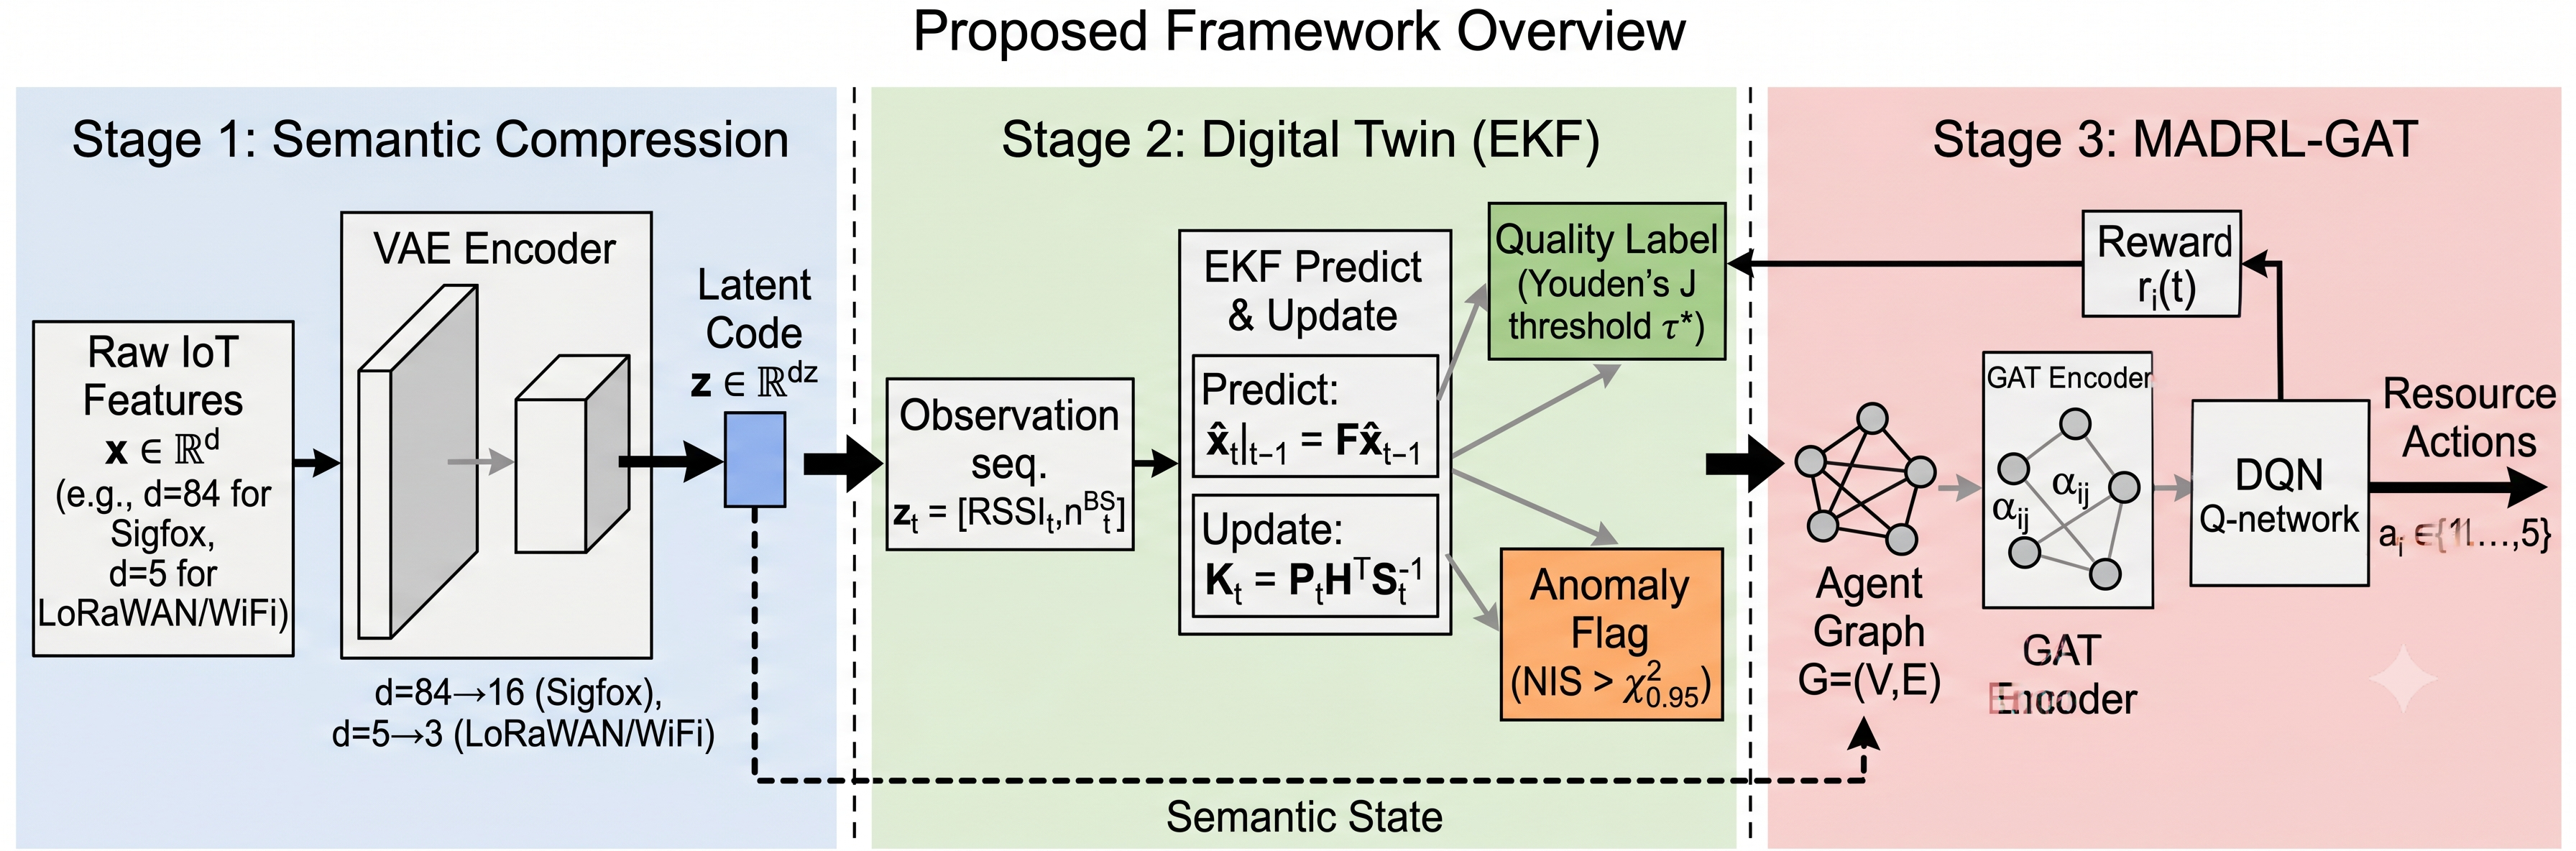
\includegraphics[width=\textwidth]{framework_overview}
    \caption{Overall architecture of the proposed three-stage framework.
    \textbf{Stage~1}: VAE compresses high-dimensional raw IoT features into
    a compact semantic latent code $\mathbf{z}$.
    \textbf{Stage~2}: The EKF-based Digital Twin estimates the channel state
    from observations $[{\rm RSSI}_t, n^{\rm BS}_t]$ and simultaneously
    outputs a connection quality label and an anomaly flag.
    \textbf{Stage~3}: MADRL-GAT agents receive $\mathbf{z}$ as state and
    cooperatively learn a resource allocation policy guided by the Digital
    Twin quality feedback.}
    \label{fig:framework}
\end{figure}

The framework operates as follows. First, the VAE is pre-trained offline on
the raw feature matrix and its encoder is frozen. At runtime, each new
IoT observation $\mathbf{x}_t$ is projected to the latent code
$\hat{\mathbf{z}}_t = \bm{\mu}_\phi(\mathbf{x}_t)$, which serves as the
state input for the MADRL agents. In parallel, the observation sequence
$[{\rm RSSI}_t, n^{\rm BS}_t]$ feeds the EKF Digital Twin, which provides
real-time quality classification and anomaly detection. The three stages
are described in detail below.

% =============================================================================
\section{Stage 1: Semantic Feature Compression via VAE}
\label{sec:vae}
% =============================================================================

\subsection{Motivation}

Raw IoT feature vectors are high-dimensional and contain redundant
information. For Sigfox Antwerp, each transmission is characterised by
RSSI readings from up to 84 base stations. Feeding such high-dimensional
inputs directly to a reinforcement learning agent is inefficient and
leads to slow convergence. A Variational Autoencoder (VAE) addresses
this by learning a compact, structured latent representation that
captures the semantically relevant variation in the data.

\subsection{Model Architecture}

% -----------------------------------------------------------------------
% FIGURE 2 — Kiến trúc VAE
% ► TỰ VẼ: encoder (FC → BN → ReLU → FC → BN → ReLU → mu/logvar)
%           reparameterisation (z = mu + eps*sigma)
%           decoder (FC → ReLU → FC → ReLU → FC → Sigmoid)
%   Ghi chú kích thước: d → 64 → 32 → dz (encoder), dz → 32 → 64 → d (decoder)
%   Với: d=84, dz=16 (Antwerp); d=5, dz=3 (LoRaWAN, Indoor)
% -----------------------------------------------------------------------
\begin{figure}[H]
    \centering
    
\includegraphics[width=0.85\textwidth]{vae_architecture}
    \caption{VAE encoder–decoder architecture.
    The encoder maps input $\mathbf{x}\in\mathbb{R}^d$ through two
    fully-connected layers (with BatchNorm and ReLU) to the distribution
    parameters $(\bm{\mu}_\phi, \log\bm{\sigma}^2_\phi)$.
    The decoder reconstructs $\hat{\mathbf{x}}$ from a sampled latent
    $\mathbf{z}\in\mathbb{R}^{d_z}$.
    Compression ratios: $84\!\to\!16$ (Antwerp), $5\!\to\!3$
    (LoRaWAN, Indoor).}
    \label{fig:vae_arch}
\end{figure}

Let $\mathbf{x}\in\mathbb{R}^d$ be the normalised input feature vector.
The VAE learns a probabilistic encoder
$q_\phi(\mathbf{z}|\mathbf{x}) = \mathcal{N}(\bm{\mu}_\phi(\mathbf{x}),\,
\mathrm{diag}(\bm{\sigma}^2_\phi(\mathbf{x})))$
and a decoder $p_\theta(\mathbf{x}|\mathbf{z})$ by maximizing the
evidence lower bound:
\begin{equation}
\mathcal{L}(\phi,\theta;\mathbf{x})
  = \underbrace{\mathbb{E}_{q_\phi}\!\left[\log p_\theta(\mathbf{x}|\mathbf{z})\right]}_{\text{reconstruction}}
  - \underbrace{\beta\, D_{\mathrm{KL}}\!\left(q_\phi(\mathbf{z}|\mathbf{x})\,\|\,
    \mathcal{N}(\mathbf{0},\mathbf{I})\right)}_{\text{regularization}},
\label{eq:elbo}
\end{equation}
where $\beta=1$ recovers the standard VAE objective (Kingma \& Welling, 2014). The reconstruction term is the mean
squared error between $\mathbf{x}$ and $\hat{\mathbf{x}}$; the KL term
regularises the latent distribution toward the standard Gaussian prior.

A latent sample during training is drawn via the reparameterisation trick
to allow gradient back-propagation:
\begin{equation}
\mathbf{z} = \bm{\mu}_\phi(\mathbf{x})
           + \bm{\varepsilon}\odot\bm{\sigma}_\phi(\mathbf{x}),
\quad \bm{\varepsilon}\sim\mathcal{N}(\mathbf{0},\mathbf{I}).
\label{eq:reparam}
\end{equation}
At inference the stochastic term is dropped and the deterministic mean
\begin{equation}
\hat{\mathbf{z}} = \bm{\mu}_\phi(\mathbf{x})
\label{eq:latent}
\end{equation}
is used as the semantic latent code passed to Stage~3.

\subsection{Training and Results}

% -----------------------------------------------------------------------
% FIGURE 3 — VAE Training Loss
% ► SỬ DỤNG ẢNH TỪ results/*/plots/vae_loss.png (đổi tên)
%   figures/vae_loss_antwerp.png
%   figures/vae_loss_lorawan.png
%   figures/vae_loss_indoor.png
% -----------------------------------------------------------------------
\begin{figure}[H]
    \centering
    \begin{subfigure}[b]{0.32\textwidth}
        
\includegraphics[width=\textwidth]{vae_loss_antwerp}
        \caption{Antwerp ($84\to16$)}
    \end{subfigure}\hfill
    \begin{subfigure}[b]{0.32\textwidth}
        
\includegraphics[width=\textwidth]{vae_loss_lorawan}
        \caption{LoRaWAN ($5\to3$)}
    \end{subfigure}\hfill
    \begin{subfigure}[b]{0.32\textwidth}
        
\includegraphics[width=\textwidth]{vae_loss_indoor}
        \caption{Indoor WiFi ($5\to3$)}
    \end{subfigure}
    \caption{VAE training loss over 30 epochs.
    Solid navy line: reconstruction loss;
    dark-red dashed line: KL divergence.
    Both components converge within the first 10 epochs.}
    \label{fig:vae_loss}
\end{figure}

Table~\ref{tab:vae} summarises the compression configuration and
reconstruction quality.

\begin{table}[H]
\centering
\caption{VAE compression results on three IoT datasets}
\label{tab:vae}
\begin{tabular}{lcccc}
\toprule
\textbf{Dataset} & \textbf{Input dim $d$} & \textbf{Latent dim $d_z$}
    & \textbf{Ratio} & \textbf{Recon. MSE} \\
\midrule
Sigfox Antwerp  & 84 & 16 & $5.25\times$ & 0.0082 \\
LoRaWAN Italy   &  5 &  3 & $1.67\times$ & 0.0160 \\
Indoor WiFi     &  5 &  3 & $1.67\times$ & 0.0537 \\
\bottomrule
\end{tabular}
\end{table}

The low reconstruction MSE (especially $0.0082$ for Antwerp at a
$5.25\times$ compression ratio) confirms that the latent code faithfully
retains the channel-quality information embedded in the 84-dimensional
Sigfox fingerprint.

% =============================================================================
\section{Stage 2: EKF-Based Digital Twin}
\label{sec:dt}
% =============================================================================

\subsection{Motivation}

Static unsupervised methods (K-Means, GMM) classify connection quality
based on instantaneous feature vectors and fail when feature clusters
overlap—as observed on LoRaWAN where both methods achieve AUC~$\approx$~0.50.
A physics-inspired state estimator that models temporal dynamics
can exploit the autocorrelation structure of wireless channels to
significantly improve both quality classification and anomaly detection.

\subsection{State-Space Model}

The Digital Twin maintains a two-dimensional channel state vector
\begin{equation}
\mathbf{x}_t = \bigl[{\rm RSSI}_t,\; n^{\rm BS}_t\bigr]^\top \in \mathbb{R}^2,
\label{eq:state}
\end{equation}
comprising the mean received signal strength and the number of active
base stations. We adopt a constant-state motion model:
\begin{equation}
\mathbf{x}_{t+1} = \mathbf{F}\,\mathbf{x}_t + \mathbf{w}_t, \qquad
\mathbf{z}_t = \mathbf{H}\,\mathbf{x}_t + \mathbf{v}_t,
\label{eq:ssmodel}
\end{equation}
where $\mathbf{F} = \mathbf{H} = \mathbf{I}_2$,
$\mathbf{w}_t\sim\mathcal{N}(\mathbf{0},\mathbf{Q})$ is process noise
with $\mathbf{Q}=\sigma_Q^2\mathbf{I}$, and
$\mathbf{v}_t\sim\mathcal{N}(\mathbf{0},\mathbf{R})$ is observation noise
with $\mathbf{R}=\sigma_R^2\mathbf{I}$.

\subsection{Extended Kalman Filter Update}

The EKF framework is selected over static methods (K-Means, GMM, LOF)
for three reasons: (i)~the time-varying Kalman gain $\mathbf{K}_t$
adaptively weights observations against current uncertainty
$\mathbf{P}_{t|t-1}$; (ii)~the NIS statistic provides a chi-squared
anomaly test grounded in the filter's uncertainty model; and
(iii)~the Youden's J threshold on the filtered estimate is data-adaptive.
The \textbf{nonlinear transition} model employs a tanh mean-reversion
function for RSSI dynamics (Ornstein-Uhlenbeck-like), motivated by the
natural tendency of wireless channels to revert toward the long-term
path-loss mean:
\begin{equation}
s^{(1)}_{t+1} = s^{(1)}_t +
  \alpha\tanh\!\Bigl(\tfrac{\mu - s^{(1)}_t}{\sigma}\Bigr) + w_t,
\label{eq:tanh_transition}
\end{equation}
where $\mu$ and $\sigma$ are the dataset RSSI mean and standard deviation,
$\alpha{=}0.3$. The time-varying Jacobian
$\mathbf{F}_t[0,0] = 1 - \alpha/(\sigma\cosh^2((\mu-\hat{s}^{(1)})/\sigma))$
changes at every step — the defining characteristic of EKF.
The filter executes a \textit{predict}–\textit{update} cycle at each time
step $t$:

\vspace{4pt}
\noindent\textbf{Predict step:}
\begin{align}
\hat{\mathbf{x}}_{t|t-1} &= \mathbf{F}\,\hat{\mathbf{x}}_{t-1|t-1},
\label{eq:pred_x}\\
\mathbf{P}_{t|t-1} &= \mathbf{F}\,\mathbf{P}_{t-1|t-1}\,\mathbf{F}^\top + \mathbf{Q}.
\label{eq:pred_p}
\end{align}

\noindent\textbf{Update step:}
\begin{align}
\mathbf{y}_t &= \mathbf{z}_t - \mathbf{H}\,\hat{\mathbf{x}}_{t|t-1}
\quad\text{(innovation)},
\label{eq:innov}\\
\mathbf{S}_t &= \mathbf{H}\,\mathbf{P}_{t|t-1}\,\mathbf{H}^\top + \mathbf{R}
\quad\text{(innovation covariance)},
\label{eq:innov_cov}\\
\mathbf{K}_t &= \mathbf{P}_{t|t-1}\,\mathbf{H}^\top\,\mathbf{S}_t^{-1}
\quad\text{(Kalman gain)},
\label{eq:kgain}\\
\hat{\mathbf{x}}_{t|t} &= \hat{\mathbf{x}}_{t|t-1} + \mathbf{K}_t\,\mathbf{y}_t,
\label{eq:upd_x}\\
\mathbf{P}_{t|t} &= \bigl(\mathbf{I} - \mathbf{K}_t\,\mathbf{H}\bigr)\,\mathbf{P}_{t|t-1}.
\label{eq:upd_p}
\end{align}

\subsection{Anomaly Detection via NIS}

The Normalized Innovation Squared (NIS) statistic
\begin{equation}
\xi_t = \mathbf{y}_t^\top\,\mathbf{S}_t^{-1}\,\mathbf{y}_t
\;\sim\;\chi^2(2)
\label{eq:nis}
\end{equation}
measures how surprising the new observation $\mathbf{z}_t$ is given the
filter's prediction. Under the null hypothesis (no anomaly), $\xi_t$
follows a chi-squared distribution with two degrees of freedom. A time
step is flagged as anomalous if
\begin{equation}
\xi_t > \chi^2_{1-\alpha}(2),\quad \alpha = 0.05
\;\Rightarrow\; \chi^2_{0.95}(2) \approx 5.99.
\label{eq:anomaly_flag}
\end{equation}

\subsection{Quality Classification via Youden's J}

Let $\hat{x}^{(1)}_{t|t}$ denote the first component of $\hat{\mathbf{x}}_{t|t}$
(estimated RSSI). The ground-truth quality label is defined as
$y_t = \mathbf{1}[{\rm RSSI}_t > \tau_{\rm obs}]$, where $\tau_{\rm obs}$
is the median of the observed RSSI sequence.

Rather than applying $\tau_{\rm obs}$ directly to the smoothed estimate
(which would introduce a systematic bias from EKF filtering), we derive
an optimal threshold by maximizing the Youden's J statistic on the
receiver operating characteristic (ROC) curve of
$\hat{x}^{(1)}_{t|t}$ vs.\ $y_t$:
\begin{equation}
\tau^* = \arg\max_{\tau}\;\bigl[\mathrm{TPR}(\tau) - \mathrm{FPR}(\tau)\bigr],
\label{eq:youden}
\end{equation}
where $\mathrm{TPR}(\tau) = P(\hat{x}^{(1)} \geq \tau \mid y=1)$ and
$\mathrm{FPR}(\tau) = P(\hat{x}^{(1)} \geq \tau \mid y=0)$. The
connection is classified as good quality if
$\hat{x}^{(1)}_{t|t} \geq \tau^*$.

This data-adaptive threshold accounts for dataset-specific RSSI
distributions and the smoothing effect of the Kalman filter, without
requiring any manual calibration.

\subsection{State Estimation Results}

% -----------------------------------------------------------------------
% FIGURE 4 — Digital Twin State Estimation
% ► SỬ DỤNG ẢNH TỪ results/*/plots/dt_estimation.png (đổi tên)
%   figures/dt_estimation_antwerp.png
%   figures/dt_estimation_lorawan.png
%   figures/dt_estimation_indoor.png
% -----------------------------------------------------------------------
\begin{figure}[H]
    \centering
    \begin{subfigure}[b]{0.32\textwidth}
        
\includegraphics[width=\textwidth]{dt_estimation_antwerp}
        \caption{Antwerp\\RSSI-RMSE=3.47 dBm}
    \end{subfigure}\hfill
    \begin{subfigure}[b]{0.32\textwidth}
        
\includegraphics[width=\textwidth]{dt_estimation_lorawan}
        \caption{LoRaWAN\\RSSI-RMSE=5.50 dBm}
    \end{subfigure}\hfill
    \begin{subfigure}[b]{0.32\textwidth}
        
\includegraphics[width=\textwidth]{dt_estimation_indoor}
        \caption{Indoor WiFi\\RSSI-RMSE=2.44 dBm}
    \end{subfigure}
    \caption{Digital Twin EKF state estimation over the first 500 time steps
    on three datasets. Each subplot shows mean RSSI (upper) and number of
    active base stations (lower). Dark-gray dashed: noisy observations
    (with injected faults); solid line: EKF estimate.}
    \label{fig:dt}
\end{figure}

% =============================================================================
\section{Stage 3: MADRL with Graph Attention Network}
\label{sec:madrl}
% =============================================================================

\subsection{Multi-Agent Problem Formulation}

Consider $N=5$ IoT agents sharing a wireless medium. Each agent $i$ must
select a resource allocation action $a_i \in \{1,\ldots,A\}$ (e.g.,
transmission power level or channel index) at each time step. The
collective goal is to maximize the long-run sum of quality-weighted rewards.

Agent $i$'s local state at time $t$ is the semantic latent code produced
by Stage~1:
\begin{equation}
\mathbf{s}_i^t = \hat{\mathbf{z}}_i^t \in \mathbb{R}^{d_z}.
\label{eq:state_madrl}
\end{equation}
Agents are connected in a graph $\mathcal{G}=(\mathcal{V},\mathcal{E},\mathbf{A})$
where the adjacency matrix $\mathbf{A}$ encodes spatial proximity
(Antwerp: Gaussian kernel of GPS distances; LoRaWAN: feature correlation;
Indoor: fully-connected).

\subsection{Graph Attention Network Encoder}

Before computing an action, each agent aggregates information from its
neighbors using a two-layer GAT. For agent $i$ with neighbour set
$\mathcal{N}(i)$, the attention coefficient between $i$ and $j$ is:
\begin{align}
e_{ij} &= \mathrm{LeakyReLU}\!\left(
  \mathbf{a}^\top\!\bigl[\mathbf{W}\mathbf{h}_i \,\|\, \mathbf{W}\mathbf{h}_j\bigr]
\right), \label{eq:gat_e}\\
\alpha_{ij} &= \frac{\exp(e_{ij})}{\displaystyle\sum_{k\in\mathcal{N}(i)}\exp(e_{ik})},
\label{eq:gat_alpha}
\end{align}
where $\mathbf{W}\in\mathbb{R}^{d_h\times d_z}$ is a shared linear
projection and $\mathbf{a}\in\mathbb{R}^{2d_h}$ is a learnable attention
vector. The graph-aware embedding is:
\begin{equation}
\mathbf{h}'_i = \mathrm{ELU}\!\left(
  \sum_{j\in\mathcal{N}(i)}\alpha_{ij}\,\mathbf{W}\mathbf{h}_j
\right).
\label{eq:gat_h}
\end{equation}
Multi-head attention with $H$ heads is used at the first layer and the
outputs are concatenated; the second layer uses a single head with mean
aggregation.

\subsection{Deep Q-Network and Training}

Each agent maintains an independent Q-network $Q_i(\mathbf{h}'_i, a;\,\bm{\theta}_i)$
that estimates the expected cumulative reward for taking action $a$ in
graph-state $\mathbf{h}'_i$. The network is trained with experience
replay and a target network via the DQN loss:
\begin{equation}
\mathcal{L}(\bm{\theta}_i) =
\mathbb{E}_{\mathcal{B}}\!\left[
  \Bigl(
    r_t + \gamma\max_{a'}Q_i\!\left(\mathbf{h}'_{i,t+1},\,a';\,\bm{\theta}_i^-\right)
    - Q_i\!\left(\mathbf{h}'_{i,t},\,a_t;\,\bm{\theta}_i\right)
  \Bigr)^2
\right],
\label{eq:dqn}
\end{equation}
where $\gamma$ is the discount factor and $\bm{\theta}_i^-$ are the
periodically-copied target network parameters.

\subsection{Reward Function}

The reward received by agent $i$ at time $t$ integrates the Digital Twin
quality feedback from Stage~2:
\begin{equation}
r_i(t) = \hat{q}_i(t)\cdot\widehat{\rm RSSI}_i(t)
         - \lambda\,a_i(t)
         + \mu\,\mathbb{1}\!\bigl[\xi_i(t) < \chi^2_{0.95}(2)\bigr],
\label{eq:reward}
\end{equation}
where $\widehat{\rm RSSI}_i(t)$ is the EKF-estimated RSSI,
$\hat{q}_i(t)\in\{0,1\}$ is the quality label from Stage~2
(Eq.~\ref{eq:youden}), $\lambda>0$ penalizes unnecessary resource
consumption, and $\mu>0$ gives a bonus when no anomaly is detected. This coupling between the
Digital Twin (Stage~2) and the MADRL agent (Stage~3) constitutes the
key integration mechanism of the proposed framework.

\subsection{Complete Training Procedure}

\begin{algorithm}[H]
\caption{Proposed Framework: Training Procedure}
\label{alg:train}
\begin{algorithmic}[1]
\REQUIRE Dataset $\mathcal{D}$; config $\{d_z, \sigma_Q, \sigma_R,
         \varepsilon_0, \gamma, N_{\rm ep}\}$
\STATE \textbf{// Stage 1: VAE pre-training}
\STATE Normalize features: $\mathbf{X} \leftarrow (\mathbf{X}-\mu)/\sigma$
\FOR{epoch $e = 1$ \textbf{to} $E_{\rm VAE}$}
  \STATE Update $(\phi,\theta)$ by minimizing $-\mathcal{L}$ in Eq.~(\ref{eq:elbo})
\ENDFOR
\STATE Freeze encoder; extract $\hat{\mathbf{Z}} = \bm{\mu}_\phi(\mathbf{X})$
\STATE \textbf{// Stage 2: Digital Twin calibration}
\STATE Set adaptive threshold $\tau_{\rm obs} \leftarrow \mathrm{median}({\rm RSSI})$
\STATE Run EKF on $\{[{\rm RSSI}_t, n^{\rm BS}_t]\}_{t=1}^{N}$
       (Eqs.~\ref{eq:pred_x}--\ref{eq:upd_p})
\STATE Compute $\tau^* \leftarrow \arg\max_\tau[\mathrm{TPR}(\tau)-\mathrm{FPR}(\tau)]$
       via Eq.~(\ref{eq:youden})
\STATE \textbf{// Stage 3: MADRL-GAT training}
\STATE Initialise $\{Q_i, \mathcal{B}_i\}_{i=1}^N$; $\varepsilon \leftarrow \varepsilon_0$
\FOR{episode $e = 1$ \textbf{to} $N_{\rm ep}$}
  \FOR{each time step $t$}
    \STATE Compute GAT embeddings $\{\mathbf{h}'_i\}$ via Eqs.~(\ref{eq:gat_e})--(\ref{eq:gat_h})
    \STATE Select $a_i \leftarrow \varepsilon$-greedy w.r.t.\ $Q_i$
    \STATE Observe reward $r_i(t)$ (Eq.~\ref{eq:reward}) and next state
    \STATE Store in $\mathcal{B}_i$; update $Q_i$ via Eq.~(\ref{eq:dqn})
  \ENDFOR
  \STATE Decay $\varepsilon$; soft-update target networks $\bm{\theta}_i^-$
\ENDFOR
\end{algorithmic}
\end{algorithm}

% =============================================================================
\section{Summary of Contributions}
\label{sec:summary}
% =============================================================================

Table~\ref{tab:contrib} summarises the three technical contributions and
their mapping to the three stages of the framework.

\begin{table}[H]
\centering
\caption{Summary of contributions and corresponding framework stages}
\label{tab:contrib}
\setlength{\tabcolsep}{4pt}
\begin{tabular}{>{\raggedright\arraybackslash}p{0.05\textwidth}
                >{\raggedright\arraybackslash}p{0.18\textwidth}
                >{\raggedright\arraybackslash}p{0.34\textwidth}
                >{\raggedright\arraybackslash}p{0.30\textwidth}}
\toprule
\textbf{Stage} & \textbf{Component} & \textbf{Technical Novelty}
    & \textbf{Key Quantitative Result} \\
\midrule
1 & VAE Semantic Compression
  & Introduces a \textit{decoupled} semantic feature-space abstraction
    trained offline via $\beta$-VAE ELBO to minimize downstream MARL
    state dimensionality without joint-gradient instability; frozen
    encoder propagates $\hat{\mathbf{z}}=\bm{\mu}_{\phi^*}(\mathbf{x})$
    to Phase~2
  & MSE $\leq 0.054$; dimensional reduction up to $5.25\times$
    ($84\!\to\!16$) while fully preserving discriminative channel features \\
\midrule
2 & EKF Digital Twin
  & Achieves \textit{joint} connection quality classification
    (adaptive Youden's~J threshold on $\widehat{\rm RSSI}_{t|t}$)
    and real-time anomaly detection (bivariate NIS $\chi^2$ test)
    within a single low-latency filter pass; nonlinear tanh
    transition Jacobian $\mathbf{F}_t$ changes each step (genuine EKF)
  & Quality AUC up to $0.972$; Anomaly AUC up to $0.987$;
    outperforms static K-Means by up to $+80.4\%$ on LoRaWAN \\
\midrule
3 & MADRL-GAT Resource Allocation
  & Introduces a cross-layer coupling mechanism that feeds
    real-time physical-layer quality labels and anomaly flags
    from the Digital Twin directly into a graph-attention-driven
    multi-agent reward $r_i(t)$
  & Stable cooperative policy convergence within $50$ training
    episodes across all environments; maximum evaluation reward
    of $3{,}089$ \\
\bottomrule
\end{tabular}
\end{table}

\end{document}
